\documentclass[pdf]{beamer}
\usepackage{svg}
\usepackage{tikz}
\usepackage{amsmath,mathtools,amssymb,amsfonts}
\usepackage{pgfplots}


\title{Simple Linear Regression}
\logo{\includesvg[width=1.2cm]{../NBU}}
\author[Bhaya, A.G.]{Bhaya, A.G.}

\usetheme{Berkeley}
\usecolortheme{default}

\newcounter{myproblem}
\newenvironment{prob}{
  \stepcounter{myproblem}
  \begin{exampleblock}{Problem \themyproblem}
}{
  \end{exampleblock}
}

\pgfplotsset{compat=1.18}
\begin{document}
    \begin{frame}
        \maketitle
    \end{frame}

    \begin{frame}{Contents}
        \tableofcontents
    \end{frame}

    \section{Simple Linear Regression}
    \begin{frame}{Simple Linear Regression}
        \begin{definition}
            \textbf{Simple linear regression} is a statistical method which is used to model the relationship between two variables, one independent variable, called predictor (usually \(x\)), and another dependent variable, called outcome (usually \(y\)).
        \end{definition}

        Linear regression basically tries to find the best-fit line that predicts \(y\) from \(x\).
    \end{frame}

    \subsection{Example: Simple Linear Regression}
    \begin{frame}{Example: Simple Linear Regression}
        Let us consider an example.

        \begin{example}
            Considering we have to predict the score a student might get in a test based on the total hours he studied for it the night before.
        \end{example}

        Say, we model the relationship between score (\(y\)), and duration of study (\(x\)) using \(y=5x+50\). This means the base score he might get is 50, which increases by 5 points for each hour that he studies.
    \end{frame}

    \subsection{Goal of Simple Linear Regression}
    \begin{frame}{Goal of Simple Linear Regression}
        The one and only goal of simple linear regression is to model the relationship through a best-fit line, which predicts the outcome based on the predictor. The best-fit line is selected such that it minimizes the difference between actual values and the predicted values.

        This method of creating the best-fit line which minimizes the difference between actual and predicted values is called the \textbf{least squares method}.
    \end{frame}

    \begin{frame}{A Best-Fit Line}
        
        \begin{figure}[h!]
        \centering
        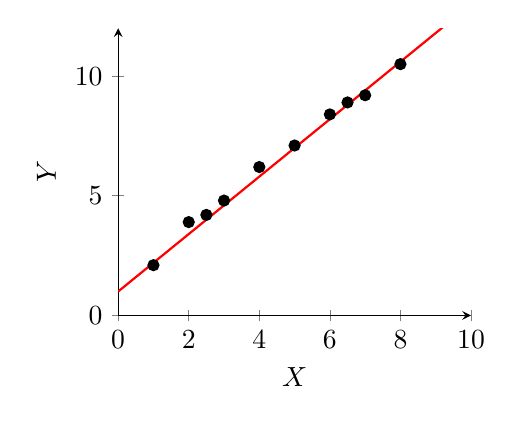
\begin{tikzpicture}
        \begin{axis}[
            axis lines = left,
            xlabel = $X$,
            ylabel = $Y$,
            xmin=0, xmax=10,
            ymin=0, ymax=12,
            grid=none,
            width=0.5\textwidth
        ]
        
        % Random sample points
        \addplot[
            only marks,
            mark=*,
        ] coordinates {
            (1,2.1)
            (2,3.9)
            (3,4.8)
            (4,6.2)
            (5,7.1)
            (6,8.4)
            (7,9.2)
            (8,10.5)
            (2.5,4.2)
            (6.5,8.9)
        };
        
        % Best fit line (approximate)
        \addplot[
            domain=0:10,
            samples=100,
            thick,
            red,
        ] {1 + 1.2*x};
        
        \end{axis}
        \end{tikzpicture}
        \caption{A best-fit line between scattered data plots.}
        \label{fig:linear-regression}
        \end{figure}

        \begin{block}{Remark}
            A best-fit line \textbf{may not} pass through all the points.
        \end{block}
    \end{frame}

    \section{Loss Function in Linear Regression}

    \begin{frame}{Loss Function in Linear Regression}
        Loss function in linear regression is defined by the mean squared error. Considering \(y_i\) to be the actual values, and \(\hat{y}_i\) to be the predicted values, where \(\hat{y}_i=wx+b\), the loss function \(L(w)\) is,

        \begin{equation}\label{eq:1}
            L(w)=\frac{1}{n}\sum_{i=1}^n{(y_i-\hat{y}_i)^2}=\frac{1}{n}\sum_{i=1}^n{\{y_i-(wx_i+b)\}^2}
        \end{equation}

        We find the best-fit line, by minimizing the loss function shown in equation \eqref{eq:1}.
    \end{frame}

    \section{Minimizing the Loss Function}
    \begin{frame}{Minimizing the Loss Function}
        There are two approaches, one might take to minimize the loss function,

        \begin{enumerate}
            \item Calculus
            \item Linear Algebra
        \end{enumerate}

        Further lectures will solve ML problems by applying linear algebra, but you my use either of the approaches when it comes to solving these problems.
    \end{frame}

    \subsection{Minimization: Calculus Approach}
    \begin{frame}{Minimization: Calculus Approach}
        To find the best-fit line, we minimize the loss function given in equation \eqref{eq:1}, i.e., we equate \(\nabla_wL(w)=0\), and \(\nabla _b L(w)=0\).

        \begin{align}
            \nabla_bL(w)&=\frac{\partial}{\partial b}\frac{1}{n}\sum_{i=1}^n{\{y_i-(wx_i+b)\}^2}=0 \nonumber\\
            &\Rightarrow \sum_{i=1}^n(y_i-wx_i-b)=0 \nonumber\\
            &\Rightarrow \sum_{i=1}^nb=\sum_{i=1}^ny_i-w\sum_{i=1}^nx_i\nonumber\\
            &\Rightarrow \boxed{b^*=\frac{\sum y_i}{n}-w\frac{\sum x_i}{n}=\overline{y}-w\overline{x}}\label{eq:2}
        \end{align}
    \end{frame}

    \begin{frame}
        Now we minimize \(L(w)\) using, \(\nabla_w L(w)=0\)

        \begin{align}
            \nabla_wL(w)&=\frac{\partial}{\partial w}\frac{1}{n}\sum_{i=1}^n{\{y_i-(wx_i+b)\}^2}=0 \nonumber\\
            &\Rightarrow \sum_{i=1}^nx_i(y_i-wx_i-b)=0 \nonumber\\
            &\Rightarrow\sum_{i=1}^nx_i\{(y_i-\overline{y})-w(x_i-\overline{x})\}=0\nonumber\\
            &\Rightarrow\boxed{w^*=\frac{\sum(y_i-\overline{y})x_i}{\sum(x_i-\overline{x})x_i}}\label{eq:3}
        \end{align}
    \end{frame}

    \begin{frame}
        Now when we plug, \(b^*\), and \(w^*\) calculated using equations \eqref{eq:2} and \eqref{eq:3}, we get the best-fit line of equation, \(\hat y=w^*x+b^*\), where the predictions \(\hat y\) using \(x\) has the least error.
    \end{frame}

    \subsection{Minimization: Linear Algebra}
    \begin{frame}{Minimization: Linear Algebra}
        Consider a set of points \(D=\{(x_1,y_1),(x_2,y_2),\ldots,(x_n,y_n)\}\). For linear regression involving two variables, we consider,

        \begin{align*}
            A&=\begin{bmatrix}
            x_1&1\\
            x_2&1\\
            \vdots\\
            x_n&1
        \end{bmatrix}\textnormal{, }
        b=\begin{bmatrix}
            y_1\\
            y_2\\
            \vdots\\
            y_n
        \end{bmatrix}\textnormal{, and }
        x=\begin{bmatrix}
            w^*\\
            b^*
        \end{bmatrix}
        \end{align*}

        \begin{alertblock}{Careful}
            Do not mix, \(x\) with \(x_i\), and \(b\) with \(b^*\). \(x\) is the parameter matrix, and \(x_i\) are the set of predictor values. Again, \(b\) is the output vector containing \(y_i\), and \(b^*\) is a regressional parameter. 
        \end{alertblock}
    \end{frame}

    \begin{frame}
        Using the matrices \(A,x\text{ and }b\), we can write the loss function, \(L(w)\) as, \(L(w)=||Ax-b||^2\). Now \(||Ax-b||\) is a scalar, and we can square it by multiplying its transpose with itself. Thus, the loss function can be written as,

        \begin{equation}\label{eq:4}
            L(w)=(Ax-b)^T(Ax-b)
        \end{equation}

        Upon minimizing equation \eqref{eq:4}, we get,

        \begin{equation}\label{eq:5}
            \nabla L(w)=2(Ax-b)^TA=2A^T(Ax-b)=0
        \end{equation}

        We then get the regressional parameters, \(w^*\), and \(b^*\) by modifying equation \eqref{eq:5} as,

        \begin{equation}\label{eq:6}
            A^TAx=A^Tb
        \end{equation}
    \end{frame}

    \begin{frame}{A Simple Problem}
        \begin{prob}
            Considering regression in one dimension, so our inputs \(x_i\), and ouputs \(y_i\) are in \(\mathbb{R}\). Linny uses regular linear regression. Given the predefined dataset, \(D=\{((1),1),((2),2),((3),4),((3),2)\}\), what values of \(\theta\) and \(\theta_0\), optimize the mean squared error of hypotheses of the form \(h(x;\theta,\theta_0)=\theta x+\theta_0\)?
        \end{prob}
    \end{frame}

    \begin{frame}{Solution}
        We create our input matrix \(A\), output vector \(b\), and regressional parameter vector \(x\) as follows,

        \begin{align*}
            A=\begin{bmatrix}
                1&1\\
                2&1\\
                3&1\\
                3&1
            \end{bmatrix},\ b=\begin{bmatrix}
                1\\2\\4\\2
            \end{bmatrix}\text{, and }x=\begin{bmatrix}
                \theta\\\theta_0
            \end{bmatrix}
        \end{align*}

        Upon minimizing the loss function we get \(A^TAx=A^Tb\). Finding,

        \begin{align*}
            A^TA&=\begin{bmatrix}
                1&2&3&3\\
                1&1&1&1
            \end{bmatrix}\begin{bmatrix}
                1&1\\
                2&1\\
                3&1\\
                3&1
            \end{bmatrix}=\begin{bmatrix}
                23&9\\
                9&4
            \end{bmatrix}
        \end{align*}
    \end{frame}

    \begin{frame}
        \begin{align*}
            \text{and }A^Tb&=\begin{bmatrix}
                1&2&3&3\\
                1&1&1&1
            \end{bmatrix}\begin{bmatrix}
                1\\2\\4\\2
            \end{bmatrix}=\begin{bmatrix}
                23\\9
            \end{bmatrix}
        \end{align*}

        To find \(x\), we create the augmented matrix,

        \begin{align*}
            \left[\begin{array}{cc|c}
                 23&9&23  \\
                 9& 4&9 
            \end{array}\right]\xrightarrow{\text{Row reduction}}\left[\begin{array}{cc|c}
                 1&0&1  \\
                 0&1&0 
            \end{array}\right]
        \end{align*}

        Thus, \(x=\begin{bmatrix}
            \theta\\\theta_0
        \end{bmatrix}=\begin{bmatrix}
            1\\0
        \end{bmatrix}\).
    \end{frame}
\end{document}